\chapter{Application Performance}
A short study of the rendering performance of our solution is conducted to check for reaching the targeted 10fps for a "simple image". As simple is a subjective term, we define the fourth iterate of \textsc{Gosper's flowsnake} to be a "simple curve" and conduct testing on it, the curve being generated as shown (no rounding).

\begin{lstlisting}[language=bash]
$ ./pfcrender lsys  --rules "L L L+R++R-L--LL-R+ R -L+RR++R+L--L-R + + - - _ _ ~ ~" --sw 2 --sl 10  --it 4 --rd 0 --ia -60 --a 60
\end{lstlisting}
\begin{figure}[ht]
	\centering
	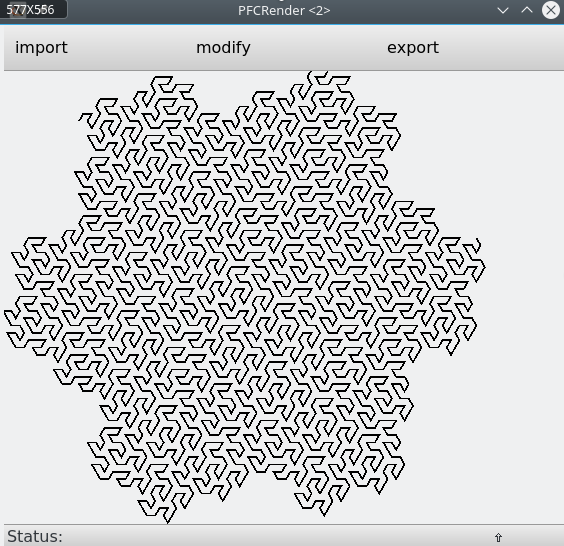
\includegraphics[width=0.8\textwidth]{simp_flosnek}
\end{figure}

Measurements are taken in an Archlinux virtual machine on an Intel Xeon E5 system at 3.5Ghz clock frequency and the program is compiled in release configuration aggressive, full program optimization.
\begin{lstlisting}
-O3 -DNDEBUG -flto=full 
\end{lstlisting}

\section{Timing Measurements}
The following measurements are taken using a slightly unwieldy shell command based on the unix \cmd{time} utility. It executes the application 100 times in batch mode and averages the reported execution times of each run.
\begin{lstlisting}
for i in {1..100}; do { time ( ./pfcrender --clear --batch lsys  --rules "L L L+R++R-L--LL-R+ R -L+RR++R+L--L-R + + - - _ _ ~ ~" --sw 2 --sl 10  --it 4 --rd 0 --ia -60 --a 60 ) } 2>&1 |tail -1| sed 's/.*  //'|cut -d" " -f1|cut -c1-4 ;done | awk '{ total += $1; count++ } END { print total/count }'
\end{lstlisting}

We compare the runtime executing different plugins in batch mode.
\begin{table}[h]
	\centering
	\begin{tabular}{r|l}
		Testcase & Application runtime[s]\\\hline
		Import only & 0.0687\\\hline
		Import \& SVG output & 0.0733\\\hline
		Import \& PDF output & 0.0761
	\end{tabular}
	\caption{Batchmode execution timings for the 4th iterate of \textsc{Gosper's flowsnake}}
\end{table}

It is apparent from these results, that the actual execution of a plugin's routine has a low impact on application runtime when the model is simple, as timings are dominated by application startup overhead. Irrespective of this effect, the proposed 10ms rendering time target is reached, even though SVG and PDF use the slow QPainter drawing engine and access the filesystem.

As the rendering time in the \gls{gui} can not be as easily benchmarked, we write a test case that triggers 100 model changed signals and reports the timing of  

